\documentclass[a4j,10pt,a4paper, fleqn]{jsarticle}\usepackage{stylefile}
%
%\usepackage{amsmath,amssymb}
\usepackage{bm}
\usepackage[dvipdfmx]{graphicx}
\usepackage{amsmath}
\graphicspath{{./fig/}}
\usepackage{subfig}
\usepackage{enumerate}
\usepackage{cite}
\usepackage{amssymb}
\usepackage{multirow}
\usepackage{color}
% \usepackage{packages/otf}


%不等号
%\usepackage{ascmac}
%\usepackage{eqnarray}
%\usepackage{hangcaption}
%
%\setlength{\textwidth}{17cm}
%\setlength{\topmargin}{-2cm}
\setlength\floatsep{0pt}
\setlength\textfloatsep{0pt}
\setlength\intextsep{0pt}
\setlength\abovecaptionskip{0pt}
%副番号を用いる場合
%\usepackage{subfigure}
%
\def\vector#1{\mbox{\boldmath $#1$}}
\newcommand{\argmax}{\mathop{\rm arg~max}\limits}
\newcommand{\argmin}{\mathop{\rm arg~min}\limits}
\newcommand{\bhline}[1]{\noalign{\hrule height #1}}

%\renewcommand{\baselinestretch}{0.997}
\begin{document}
%タイトル 2カラムぶち抜き
\twocolumn[
%titlepageは1ページ目のページ番号が出ないためカット
%	\begin{titlepage}
	\centerline{\LARGE Self-Admitted TechnicalDebtの削除}\par\vspace{1mm}
	\centerline{\LARGE およびコンテナ仮想化技術の課題に関する調査}\par\vspace{1mm}
	\centerline{\large 九州大学大学院 システム情報科学府}\par
	\centerline{\large 情報知能工学専攻 亀井研究室}\par
	\centerline{\large 修士1年 新堂 風}\par
	\centerline{\large 令和2年12月14日(月) 16:40-17:25}\par\vspace{2mm}
%	\end{titlepage}
]
%

%#! platex thesis.tex

%======================================================================
\chapter{はじめに}
\label{cha:intro}
\section{研究背景}
\label{sec:background}
Portable Health Clinic (以下,PHC)は発展途上国農村部における,健康促進のための遠隔医療システムである\cite{ahmed15:portable}.ヘルスアシスタントと呼ばれるスタッフが複数の健康測定器具を医者のいない農村部に持ち込み,村民に対して健康診断を行う.健康診断の結果,医者からの診断が必要であると判断された患者は都市部にいる医者と電話を通して繋がり,診断を受けることができる.このシステムによって,医者が直接診断できない発展途上国農村部においても人々は診断を受けることができる.このシステムでは,医者は患者を診断しながら症状や処方薬などをノートに取り,通話後にそれをコンピュータに入力して処方箋を作成する.このときにノートに書かれた手書き文字を認識し,その情報を元に処方箋を予測してコンピュータに入力する手間を削減できれば,医者の時間を節約でき,医者はさらに多くの人々の診断を行うことができる.

\section{研究目的}
本研究の目的は,遠隔医療における,処方箋予測に向けたオンライン文字認識に適したデータの拡張方法を確立することである.オープンソースのオンライン文字認識用データセットのうち,医療用語に特化したものは存在していないため,文献\cite{takahashi}では独自にデータ収集を行っている.しかしデータの収集には多くの時間と労力を要するため,文献\cite{takahashi}ではデータ拡張を行ってデータ量を水増している.***************そのため,この用語認識は学習の際のデータのとり方により認識精度にばらつきが出てしまうという問題がある.


現在,オンライン文字認識の研究においてデータ拡張を行っているものは非常に少なく,高精度を保って学習できるオンライン文字認識の拡張方法は未だ確立されていない.機械学習においてデータ量は精度を大きく左右する重要なパラメータである.オフライン文字認識については多くのデータ拡張方法が研究されているが,オンライン文字認識についてもデータの拡張方法について議論がなされるべきである.


\section{論文構成}
本論文の構成は以下の通りである.第2章では,筆者らが目指しているオンライン手書き医療用語認識,及び本研究に至った取り組むべき課題について説明を行い,既存の対策の問題点をあげる.第3章では,問題解決に向け本研究で提案する手法について説明を行う.第4章では提案手法の実装について述べる.第5章では提案手法の評価について述べる.最後に第6章で本論文のまとめと今後の展望を述べる.


\section{SATD削除期間や割合についての調査\cite{satd-removal}}

\subsection{概要}
近年では,コードからSATDを検出する手法の開発や,ソフトウェア品質への影響を調査する研究が実施されている.しかし,SATDはプロジェクト内に10年以上存在する場合もあり,これは全てのSATDが「悪い」とされているわけではなく,削除すべきSATDもあれば,削除しなくても問題ないSATDがあることも示している.
そこで文献\cite{satd-removal}では,SATDの削除に焦点を当てた研究を行っている.5つのオープンソースプロジェクトのJavaファイルについて,以下の4つのRQに基づいて調査を行っている.

\begin{itemize}
  \item RQ 1: どの程度のSATDが削除されているのか?
  \item RQ 2: 誰がSATDを削除しているのか?
  \item RQ 3: SATDはどれくらいの期間,プロジェクト内に存続するのか?
  \item RQ 4: SATDの削除はどのような活動によって行われるのか?
\end{itemize}

% ====== 結果いるのかな? ==========
% その結果,SATDの大部分は削除されており,大部分がSATDを導入した本人により削除されていたということが明らかになっている.さらに,SATDは中央値で約18日~約170日の期間で持続し,開発者はバグの修正や新機能の追加の際に,SATDを削除することが多いということが明らかになっている.

\subsection{データの前処理}
ここでは,文献\cite{satd-removal}で用いられてるデータとその事前処理について説明する.文献\cite{satd-removal}では,より多くの数・種類のSATDについて,その変化を調査するために,コメント数が多く,活動性が高いプロジェクトに焦点を当てている.選定された5つのオープンソースプロジェクト(Camel、Gerrit、Hadoop、Log4j、Tomcat)は,Javaを用いてGit上で開発されている.

\begin{figure}[t]
    \centering
    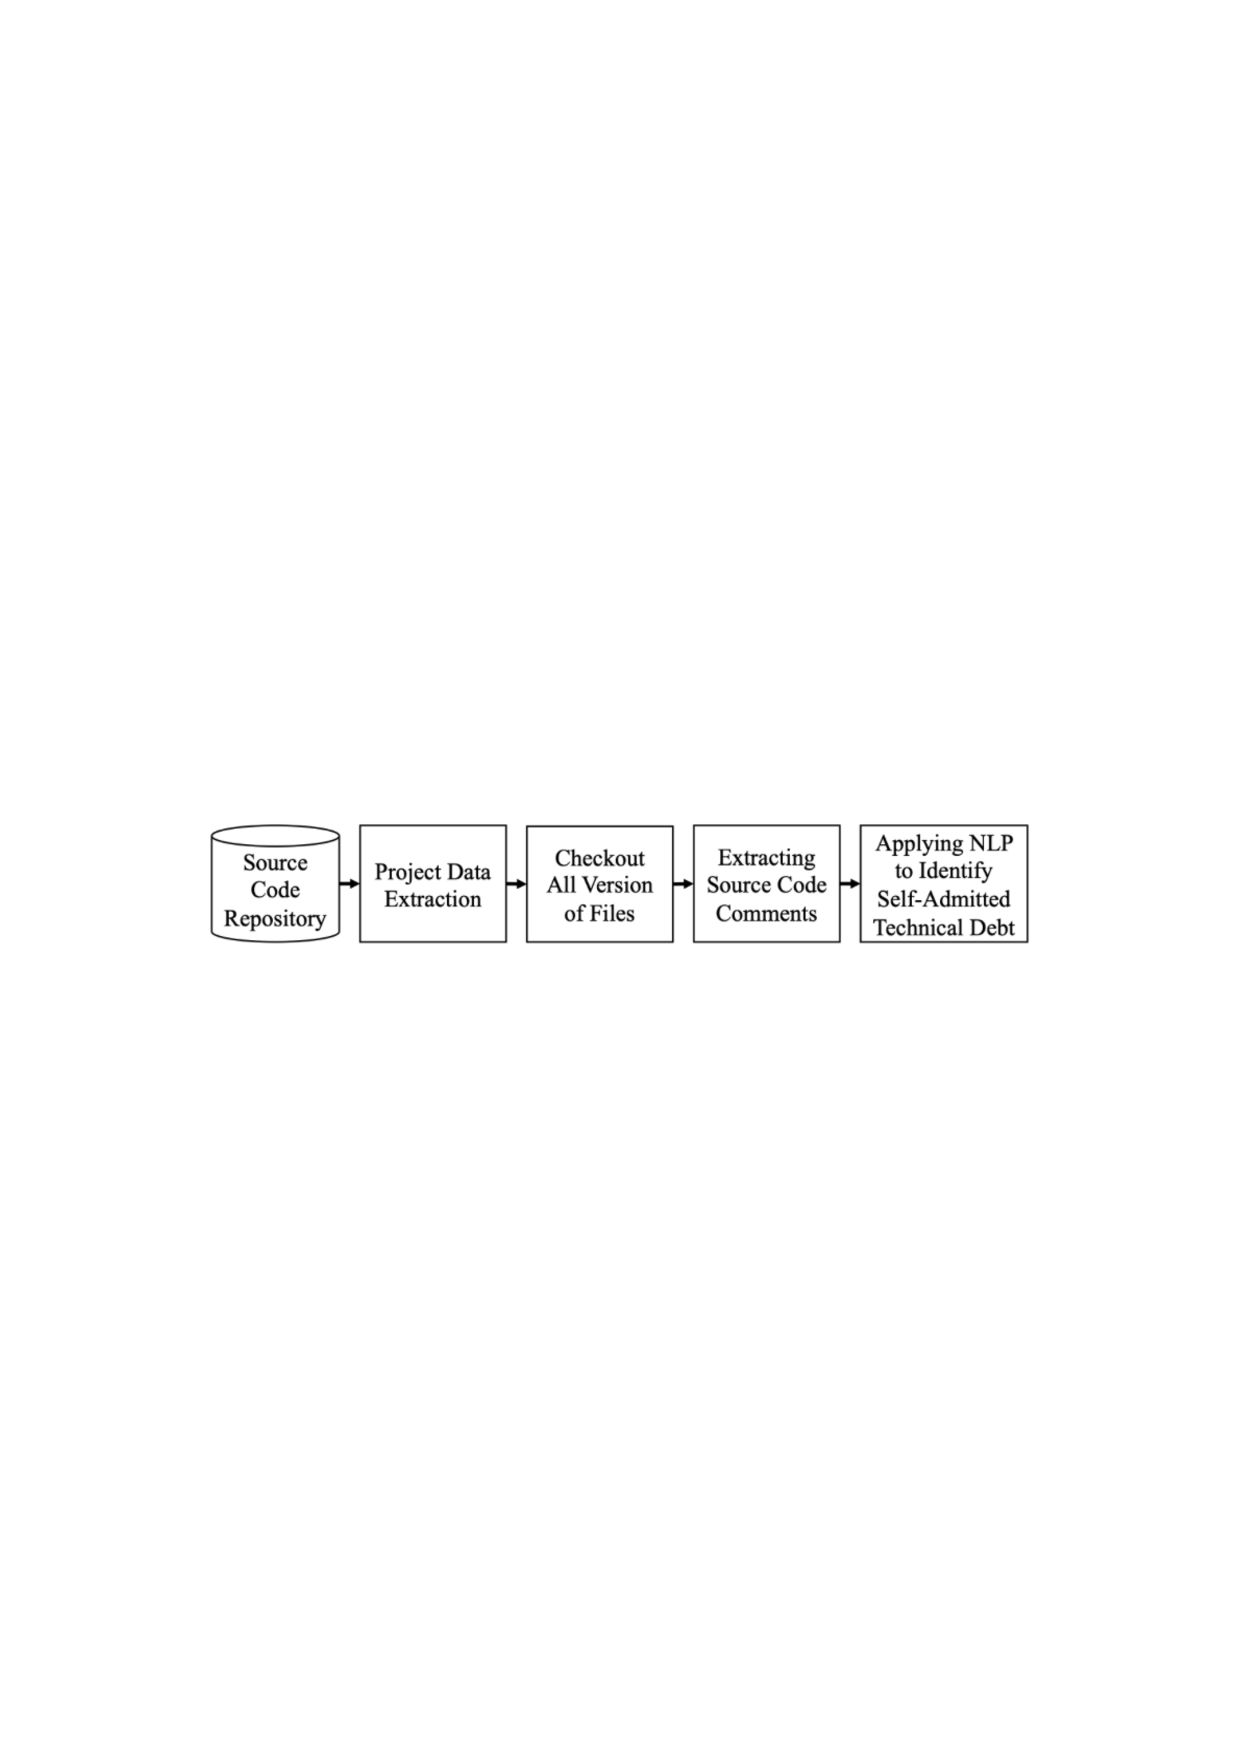
\includegraphics[width=0.9\linewidth, angle=0]{./thesis1/data-preprocess1.pdf}
    \caption{データ処理工程}
    \label{fig:1_data-preprocess}
\end{figure}

図\ref{fig:1_data-preprocess}にデータ処理の工程を示す.ExtracttingSourceCodeCommentでは,明らかに負債ではないライセンスコメントやIDEによる自動生成コメントを削除している.Applying NLP ではSATDのコメントを特定するために,Maldonadoら\cite{1-ref-25}の手法を用いている.NLP分類器は\cite{1-ref-25}によって提供されたデータを用いて訓練されたものを使用している.

各工程後に取得したデータの詳細を表\ref{fig:1_data-table},表\ref{fig:1_data-satd-table}に示す.

\begin{table*}[t]
    \centering
    \caption{調査対象プロジェクトの詳細}
    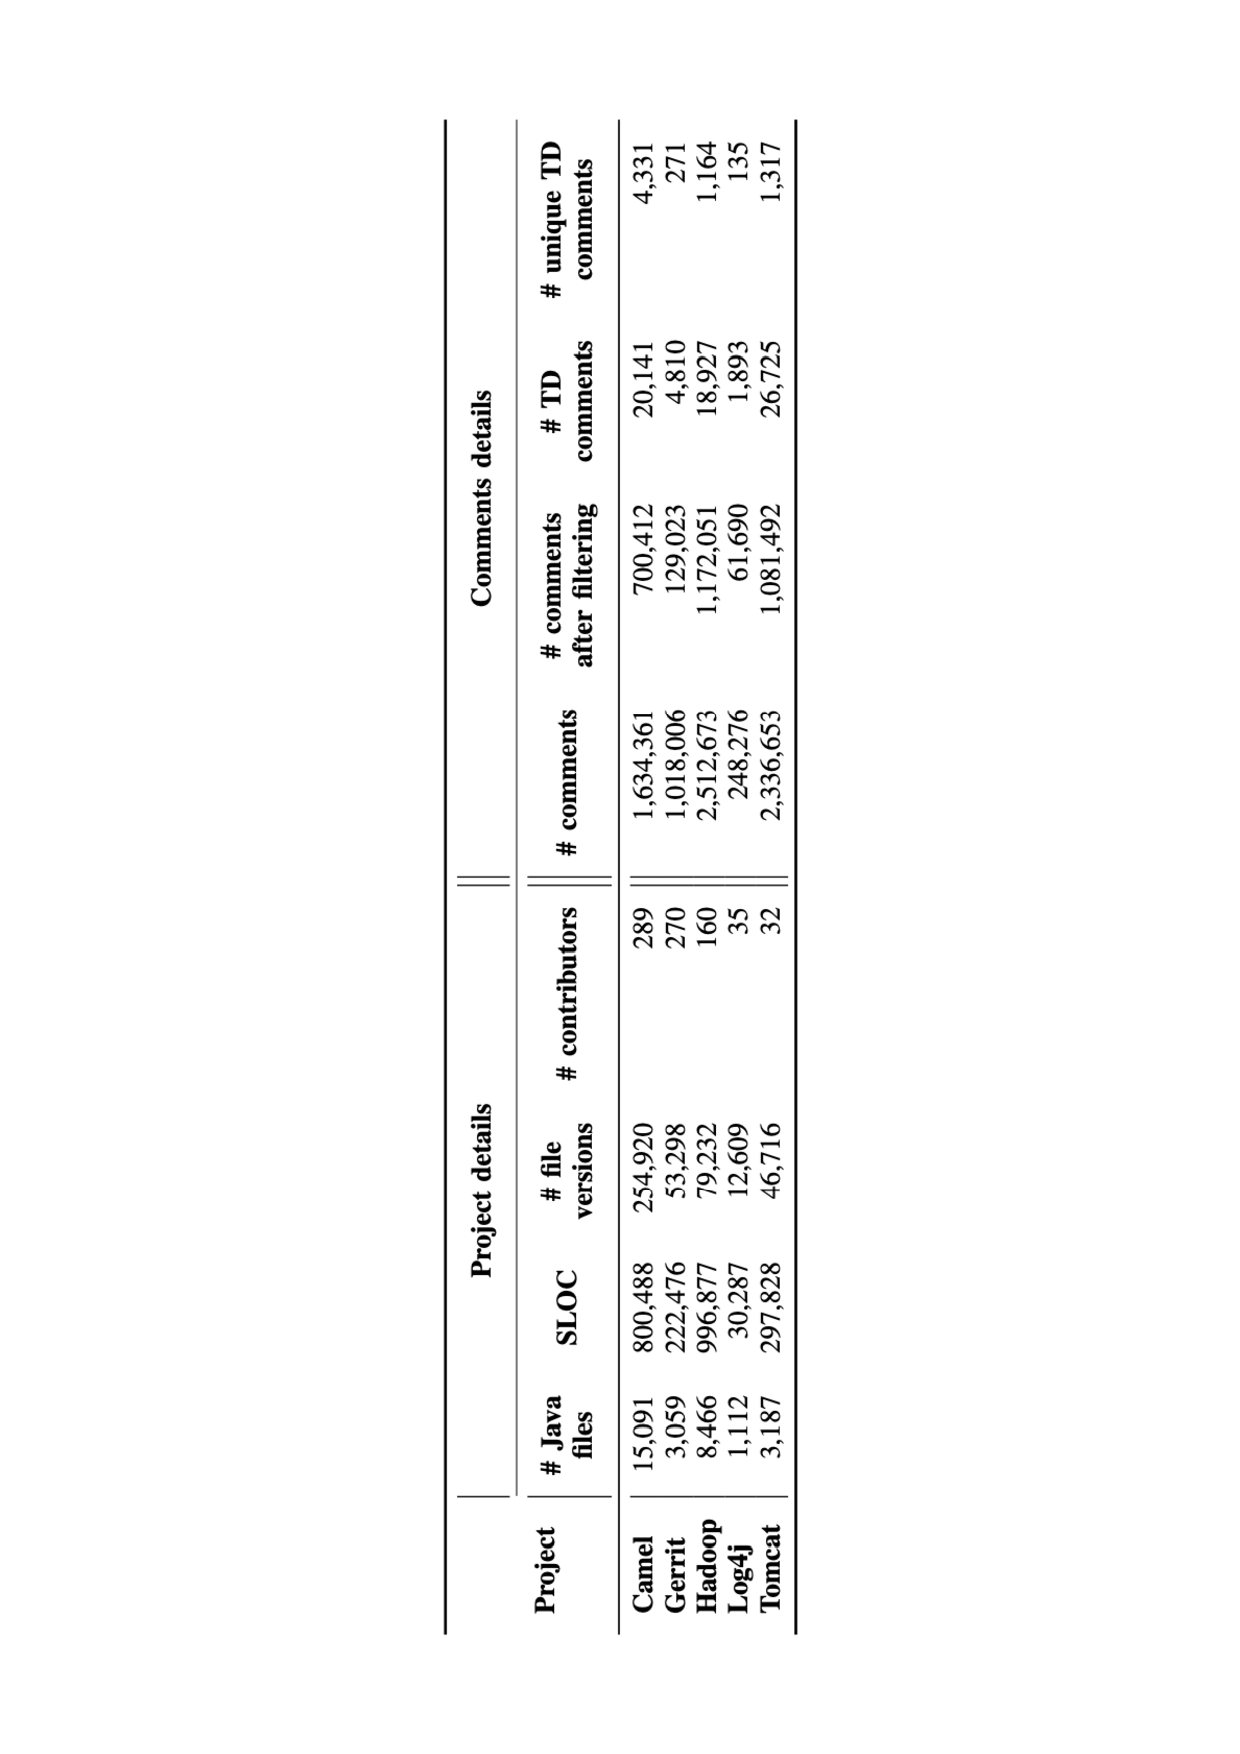
\includegraphics[height=0.9\linewidth, angle=270]{./thesis1/data-table1.pdf}
    \label{fig:1_data-table}
\end{table*}


% 全てのファイルのバージョンの特定後に,コメントを削除したコミットの日付を削除日とみなしている.また,ファイルがリネームされたり,別のフォルダに移動された場合で,古いバージョンと少なくとも90\%以上が類似している場合に,Gitはそのファイルが移動またはリネームされたファイルとして判断している.

% 技術的負債に焦点を当てるために事前に,明らかに負債ではない以下のタイプのコメントを除外する.それにより,Camelプロジェクトではコメント数を,1,634,361件から700,412件に減らしている.

% \begin{itemize}
%   \item ライセンスコメント
%   \item コメントアウトされたソースコード
%   \item IDE による自動生成コメント
%   \item Javadoc のコメント
% \end{itemize}

% SATDのコメントを特定するために,Maldonadoら\cite{1-ref-25}の手法用いている.\cite{1-ref-25}によって提供されたデータを用いて訓練されたNLP分類器を適用した結果を表\ref{fig:1_data-satd-table}に示す.


\begin{table}[t]
    \centering
    \caption{調査対象プロジェクト内SATDの詳細}
    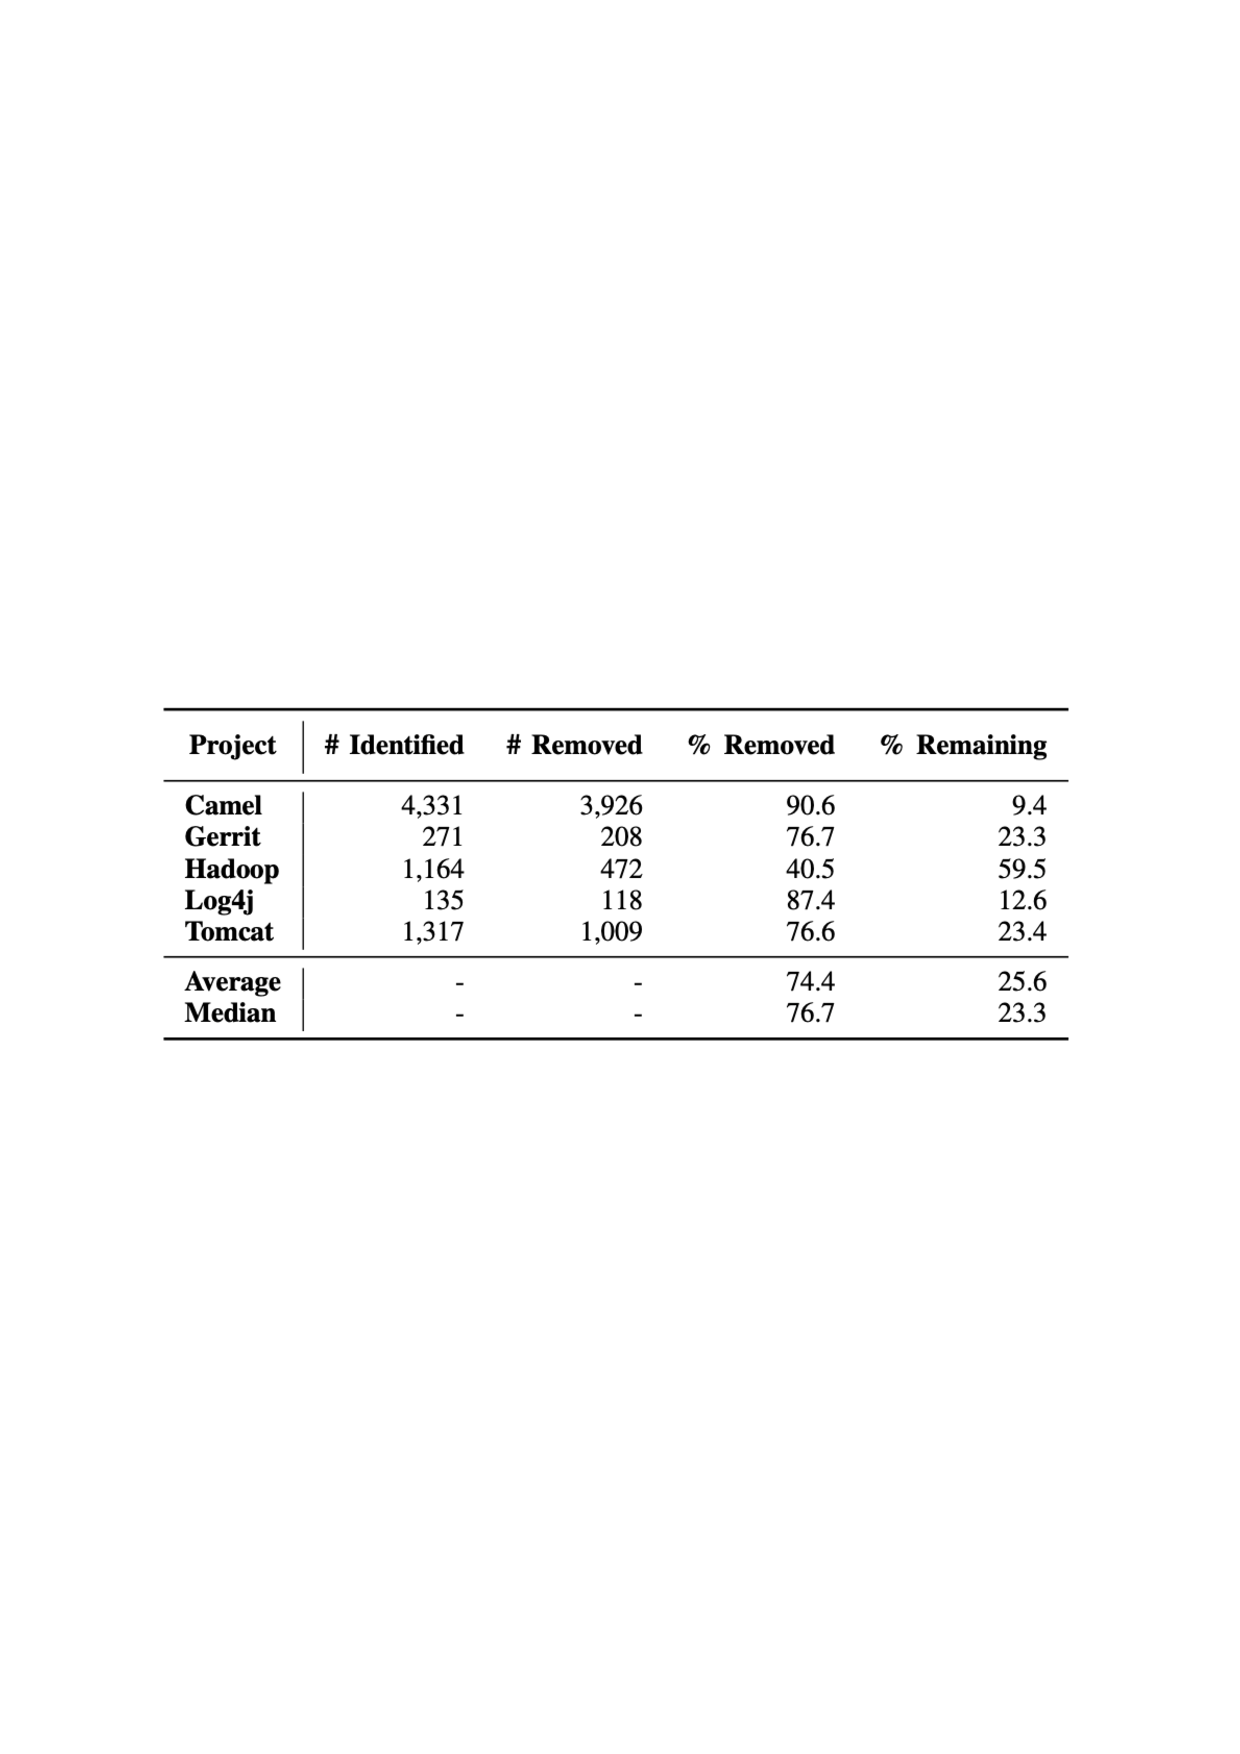
\includegraphics[width=0.9\linewidth, angle=0]{./thesis1/data-satd-table1.pdf}
    \label{fig:1_data-satd-table}
\end{table}



\subsection{結果}
以前の研究では,SATDの検出,管理,影響について検討されてきたが,そのようなSATDの削除については,ほとんど知られていなかった.文献\cite{satd-removal}では,SATDの削除について調査を行なっており,
その結果,SATDの大部分は削除され(平均74.4%),また大部分はSATDを導入した本人により削除され(平均54.4%),削除されるまでの期間は平均82~613.2日であることがわかっている.
さらに14名の開発者を対象に,SATDの導入と削除の理由について調査を実施している.調査の結果,開発者はSATDを削除する必要性を認識しているにもかかわらず,SATDを削除するための正式なプロセスはなく,ほとんどの削除はバグ修正の一環として行われていることを発見している.したがって,文献\cite{satd-removal}では,プロジェクトが効果的かつ体系的にSATDに対処できるような技術が必要であるということが示唆されている.



% ====== RQについてそれぞれで結果を書くと長くなるため削除しました ========
% \subsection{結果}
% ここでは\cite{satd-removal}のRQ1~RQ4についての結果を紹介する.

% \subsubsection{RQ1}

% 表\ref{fig:1_data-satd-table}プロジェクトごとの削除されたSATDコメントを示す.表\ref{fig:1_data-satd-table}よりSATDコメントの大部分(平均74.4\%,中央値76.7\%)が削除されていることがわかり,開発者がSATDを認識し,意識しているという傾向が示されている.

% \subsubsection{RQ2}
% 調査結果によると,ほとんどの場合SATDの大部分が,それを導入したのと同じ著者によって削除されている.平均すると,全SATD除去の54.4\%が導入した本人による削除であり,対象にした5つのプロジェクトのうち4つのプロジェクトでは自己除去が50\%以上を占めている.

% \subsubsection{RQ3}
% 一般的に,SATDがプロジェクトに留まる時間はプロジェクトによって異なり,中央値は18.2~172.8日,平均値は82~613.2日である.すべてのプロジェクトにおいて,最初の数百日でSATDは削除されており,クリティカルなSATDは急速に削除されるということが示されているが,プロジェクトにより急速に削除される期間や削除が緩やかになる期間に差がある.また,RQ2のデータをもとに,自己削除したSATDとそうでないSATDを比較し,自己削除したSATDの方が早く削除されるという結果も発見されている.



\section{SATD削除時のソースコードへの影響についての調査\cite{satd-real-removal}}
\subsection{概要}
文献\cite{satd-removal}では,SATDの削除について主に定量的な観点をもとに調査を行っているが,削除の手法についての詳細な調査は行われていなかった.SATDの削除の手法の調査を行うことで,特定の種類のSATDに対応するためのパターン学習や,それに基づいて開発者への開発手法の提供を行うことが可能になる.
文献\cite{satd-real-removal}では,\cite{satd-removal}をもとに,5つのオープンソースプロジェクトにおいてSATDがどのように削除されているかについての詳細を,以下の3つのRQに基づいて調査している.

\begin{itemize}
  \item RQ 1: SATDが削除された際の手法(クラス削除,メソッド削除など)はどのように分類されるか?
  \item RQ 2: SATDの削除はコミットメッセージに反映されているか?
  \item RQ 3: SATDを削除した際にコードにどのような変更が行われているか?
\end{itemize}

% ====== 結果いるのかな? ==========
% その結果,SATDの削除のうち「偶発的な削除(SATDの削除を目的とせずに行なった開発の中での削除)」は非常に頻繁に(最大50\%の事例)発生しておりで発生しており,実際にコミットメッセージに記録されているSATD削除の割合はかなり限られている(8\%)ことが示されている.SATDがどのように削除されるかについては,ほとんどのケースで複雑な変更が行われていることがわかり,SATDが削除されるパターンとしては,メソッド呼び出しや条件式の変更が繰り返し行われているということが明らかになっている.

\subsection{データの前処理}
文献\cite{satd-real-removal}では,文献\cite{satd-removal}で用いられてるデータを利用し,調査を行っている.

\begin{table}[t]
    \centering
    \caption{データ詳細 (出典:文献\cite{satd-real-removal})}
    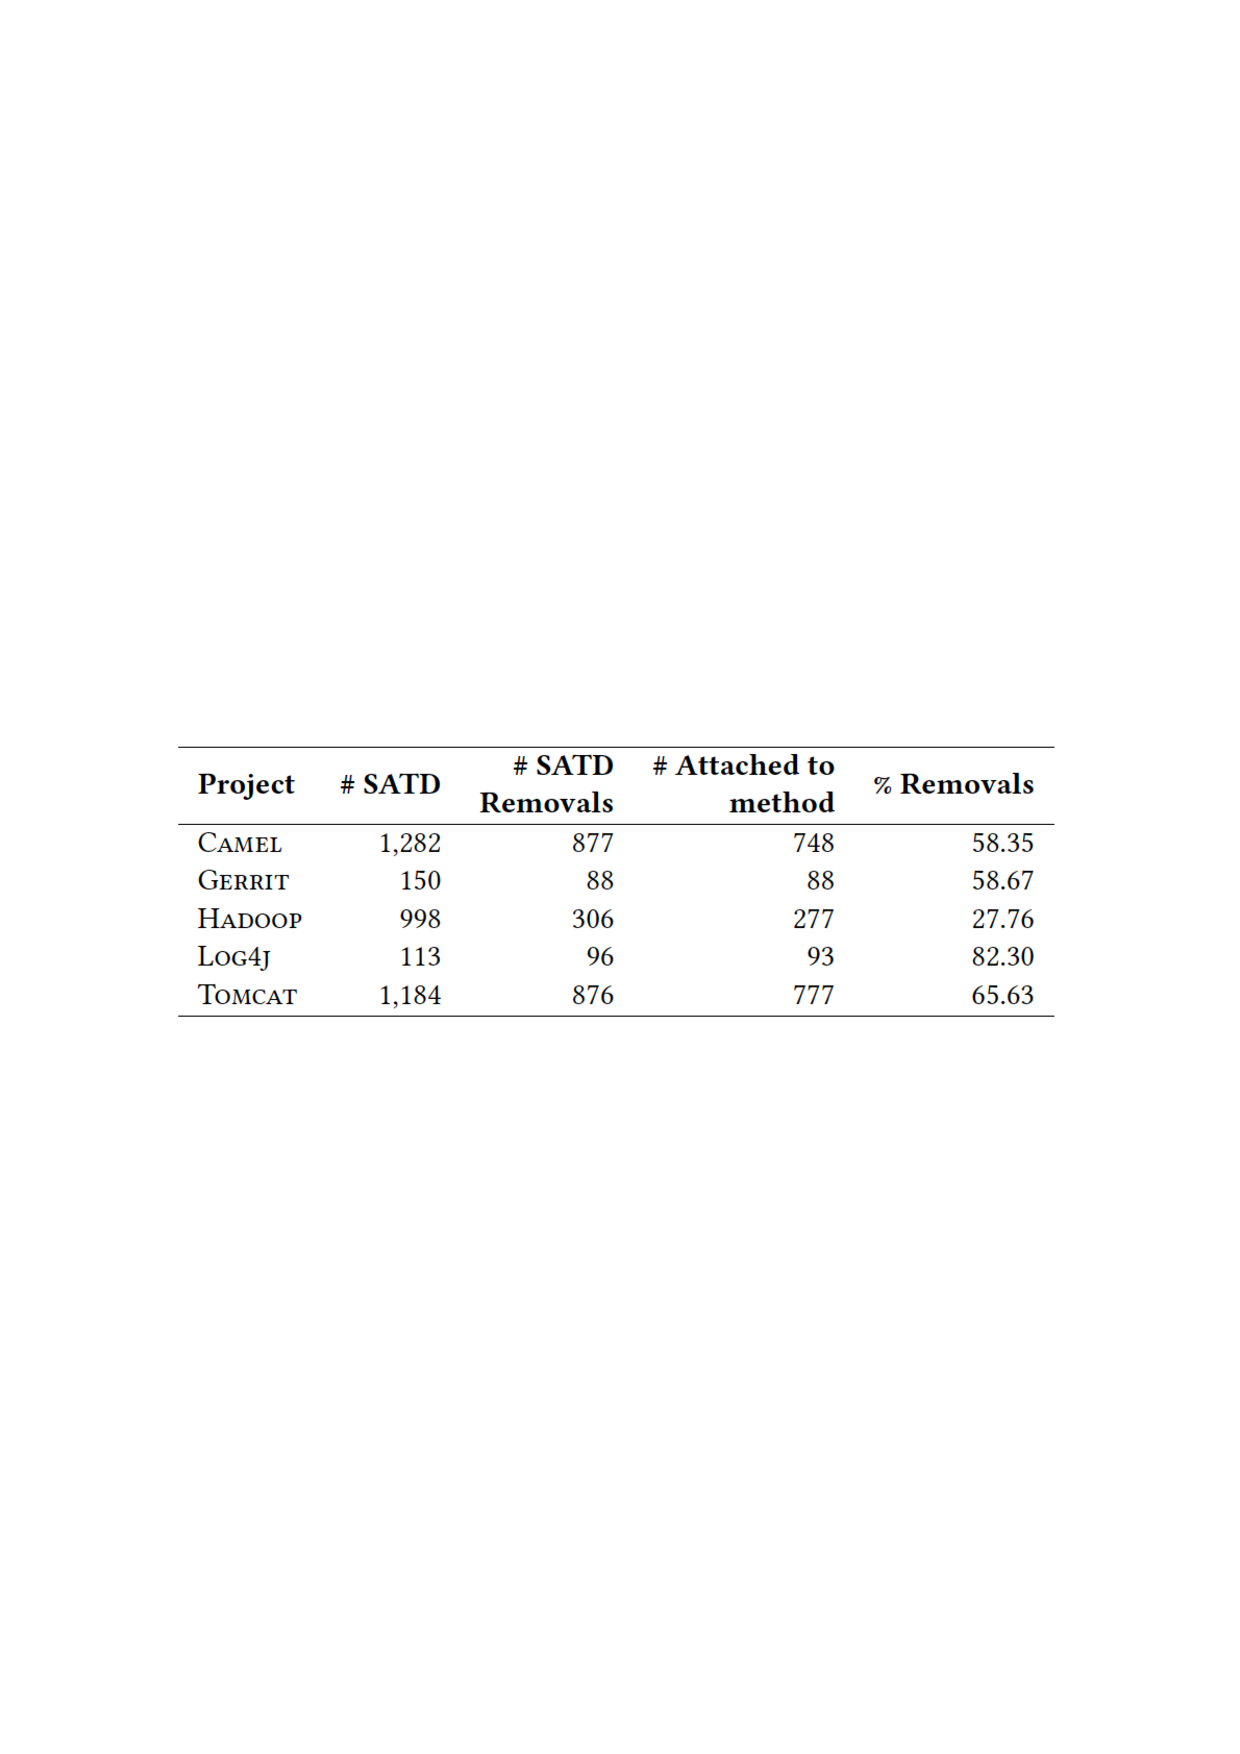
\includegraphics[width=0.9\linewidth, angle=0]{./thesis2/satd-attached-methods2.pdf}
    \label{fig:2_satd-attached-methods}
\end{table}

表\ref{fig:2_satd-attached-methods}にデータの詳細を示す.表\ref{fig:2_satd-attached-methods}では,SATDの重複や不整合を除外したため文献\cite{satd-removal}より総数が少なくなっている.

% ここらへんあんまりわかっていない
また,SATD削除の際のソースコードの変更に着目した調査を行うため,ファイルやクラス全体のSATDは無視して、メソッドレベルのSATDに着目している.
% SATDがメソッド本体に含まれていたり、メソッド定義の直前にコメントが付いていたりする場合は,SATDがメソッドに付いているとみなしている.
その後,SATDの削除として不適切な例として,(1)SATDを含むファイル名の変更が削除と判定されている場合, (2)SATDがコード内の別の場所に移動されている場合,(3)SATDが構文的に変更されたが変更後もSATDを表している場合の3パターンを除外し,表\ref{fig:2_satd-failer-alarm}にその結果を示す.

\begin{table}[t]
    \centering
    \caption{SATD 削除フィルタリング結果 (出典:\cite{satd-real-removal})}
    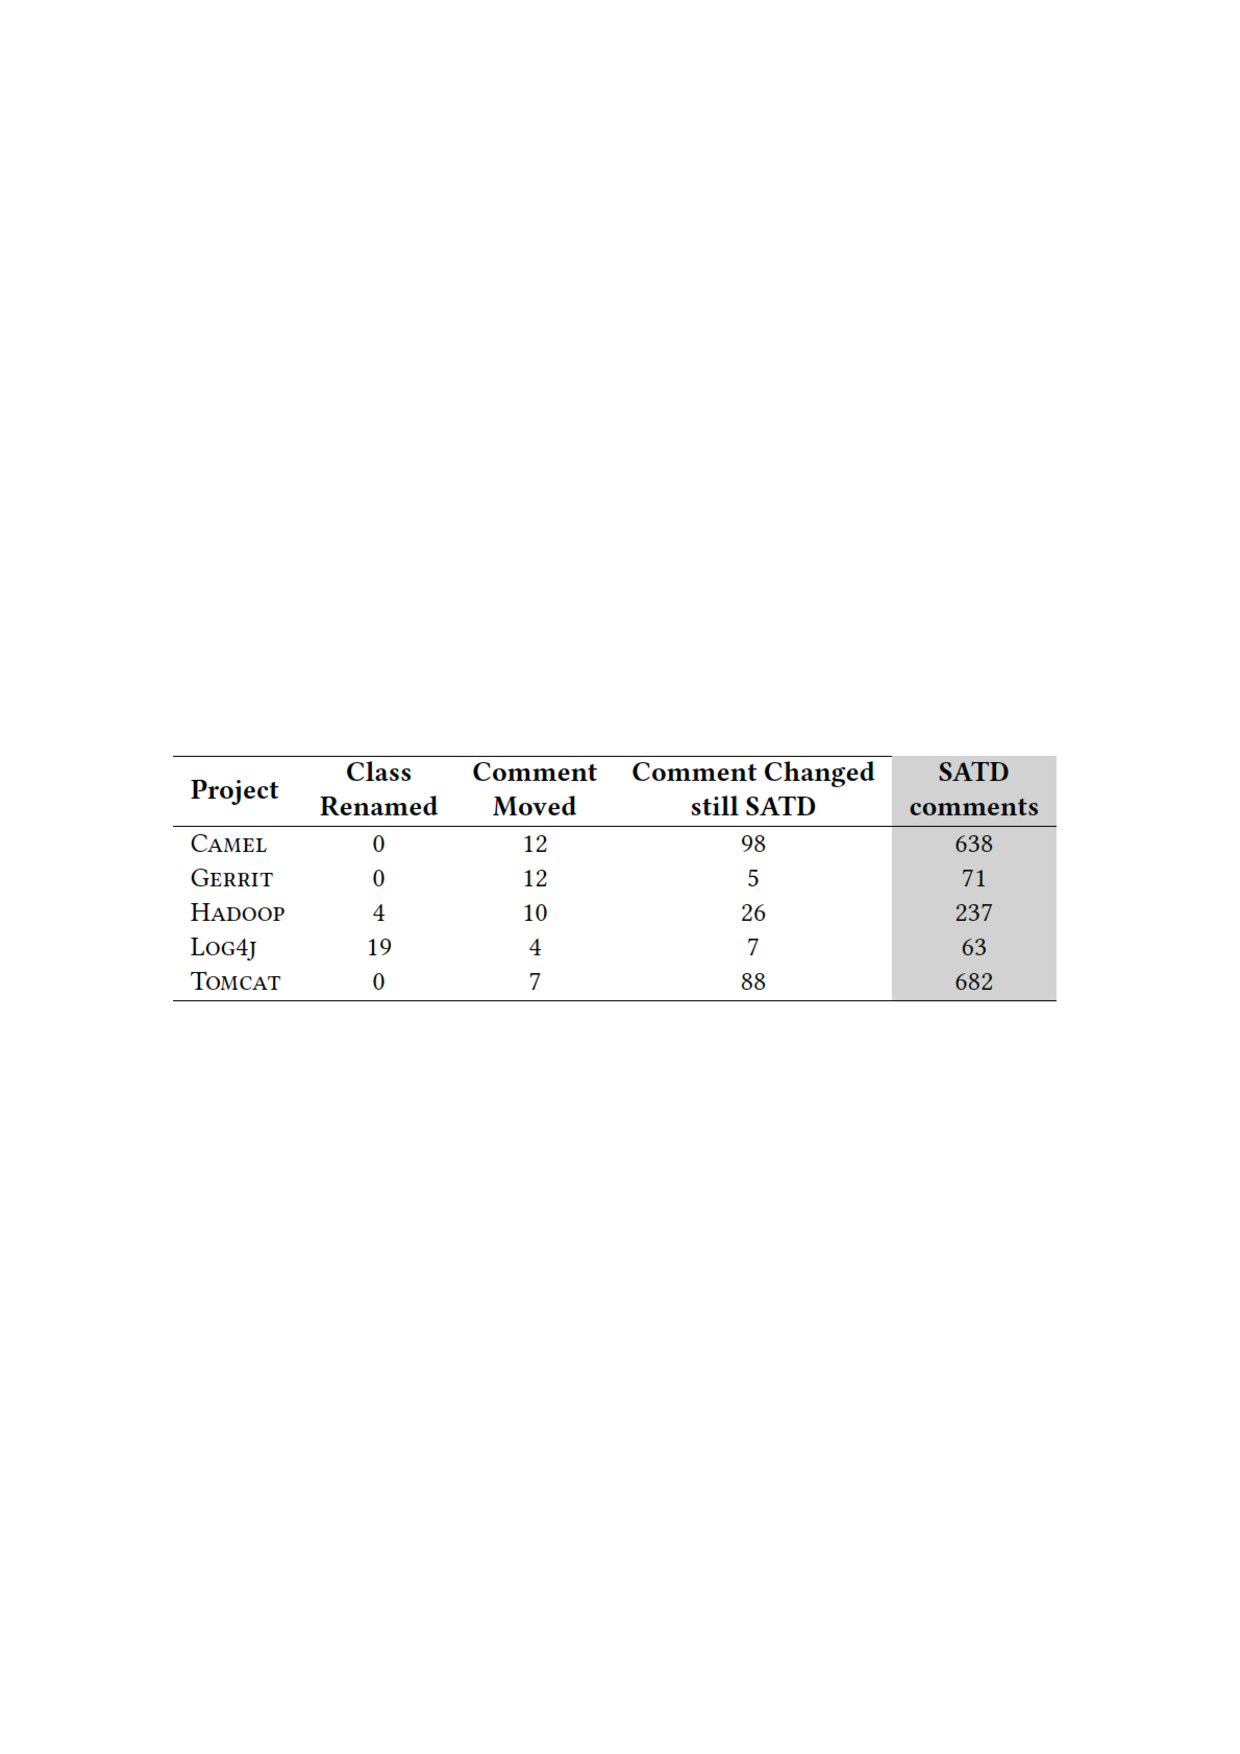
\includegraphics[width=0.9\linewidth, angle=0]{./thesis2/satd-failer-alarm2.pdf}
    \label{fig:2_satd-failer-alarm}
\end{table}

次にコミットメッセージについて,コミットメッセージがSATDの削除について言及しているかどうか判断するために,コミットメッセージと削除されたSATDとのテキストでの類似性をコサイン類似度を用いて分析し,類似している場合を手動で5段階に分類している.

\subsection{結果}
文献\cite{satd-real-removal}では,SATDの削除とソースコードの変更との関係をより深く調査している.その結果,SATDの削除はクラス全体またはメソッド全体が削除された場合に 「偶発的(SATDの削除を目的とせず)」に発生していることが明らかになっている.さらに,SATDの削除がコミットメッセージに明言されているケースは,わずか8\%であり,SATDがどのように削除されるかについては,開発者は複雑な変更を行うだけでなく,メソッドの呼び出しや条件式を変更する傾向があるということが報告されている.

文献\cite{satd-real-removal}では,これらの知見を利用して,SATD埋め込み時の推奨事項の提供や,自動アラートボットへの組み込みを通して,SATDを解決するための提案を提供することができると示唆されている.

DockerにおいてもSATDの管理,解決のために,このような推奨事項の提供やボットの開発は有効であると考えられるため,調査を行うべきである.

\section{Dockerにおけるビルドの失敗に関する調査\cite{docker-failures}}
\subsection{概要}
Dockerは近年,コンテナ型仮想化技術の世界標準として注目を浴びている.しかし,Dockerのビルドは頻繁に失敗し,その修正には長い時間を要することが度々ある.これまでの研究では,大規模開発でのDockerのビルド失敗率について調査した研究はあったが,失敗の頻度とその修正に関する調査を行った研究はほとんど存在していなかった.文献\cite{docker-failures}では,Githubにリンクされた3,828件のオープンソースプロジェクトの857,086件のDockerのビルドについて調査している.Dockerのビルドデータを用いて,以下の3つのRQについて調査を行っている.

\begin{itemize}
  \item RQ 1: Dockerのビルドはどれくらいの頻度で失敗するか?
  \item RQ 2: ビルドの修正を行うのにどれくらいの時間を要するか?
  \item RQ 3: ビルド失敗の頻度と修正時間は時間の経過によってどのような関係性があるか?
\end{itemize}

% ====== 結果いるのかな? ==========
% その結果,

\subsection{データ収集}
ここではデータの収集について説明する.文献\cite{docker-failures}では,公開されているDockerプロジェクトのビルドデータを取得するため,DockerHub APIで ``is\_autoomated"という文字列の有無をチェックして公開されているプロジェクトの特定を行っている.特定したプロジェクトからビルド数が10以下のプロジェクトをフィルタリングして,最終的に3,828件のプロジェクトのデータセット,857,086件のDockerビルドデータ(メタデータを含む)を取得している.表\ref{fig:3_docker-build-data}に各プロジェクトにおけるビルド数の統計値を示す.


\begin{table}[t]
    \centering
    \caption{各プロジェクトにおけるビルド数の基本統計}
    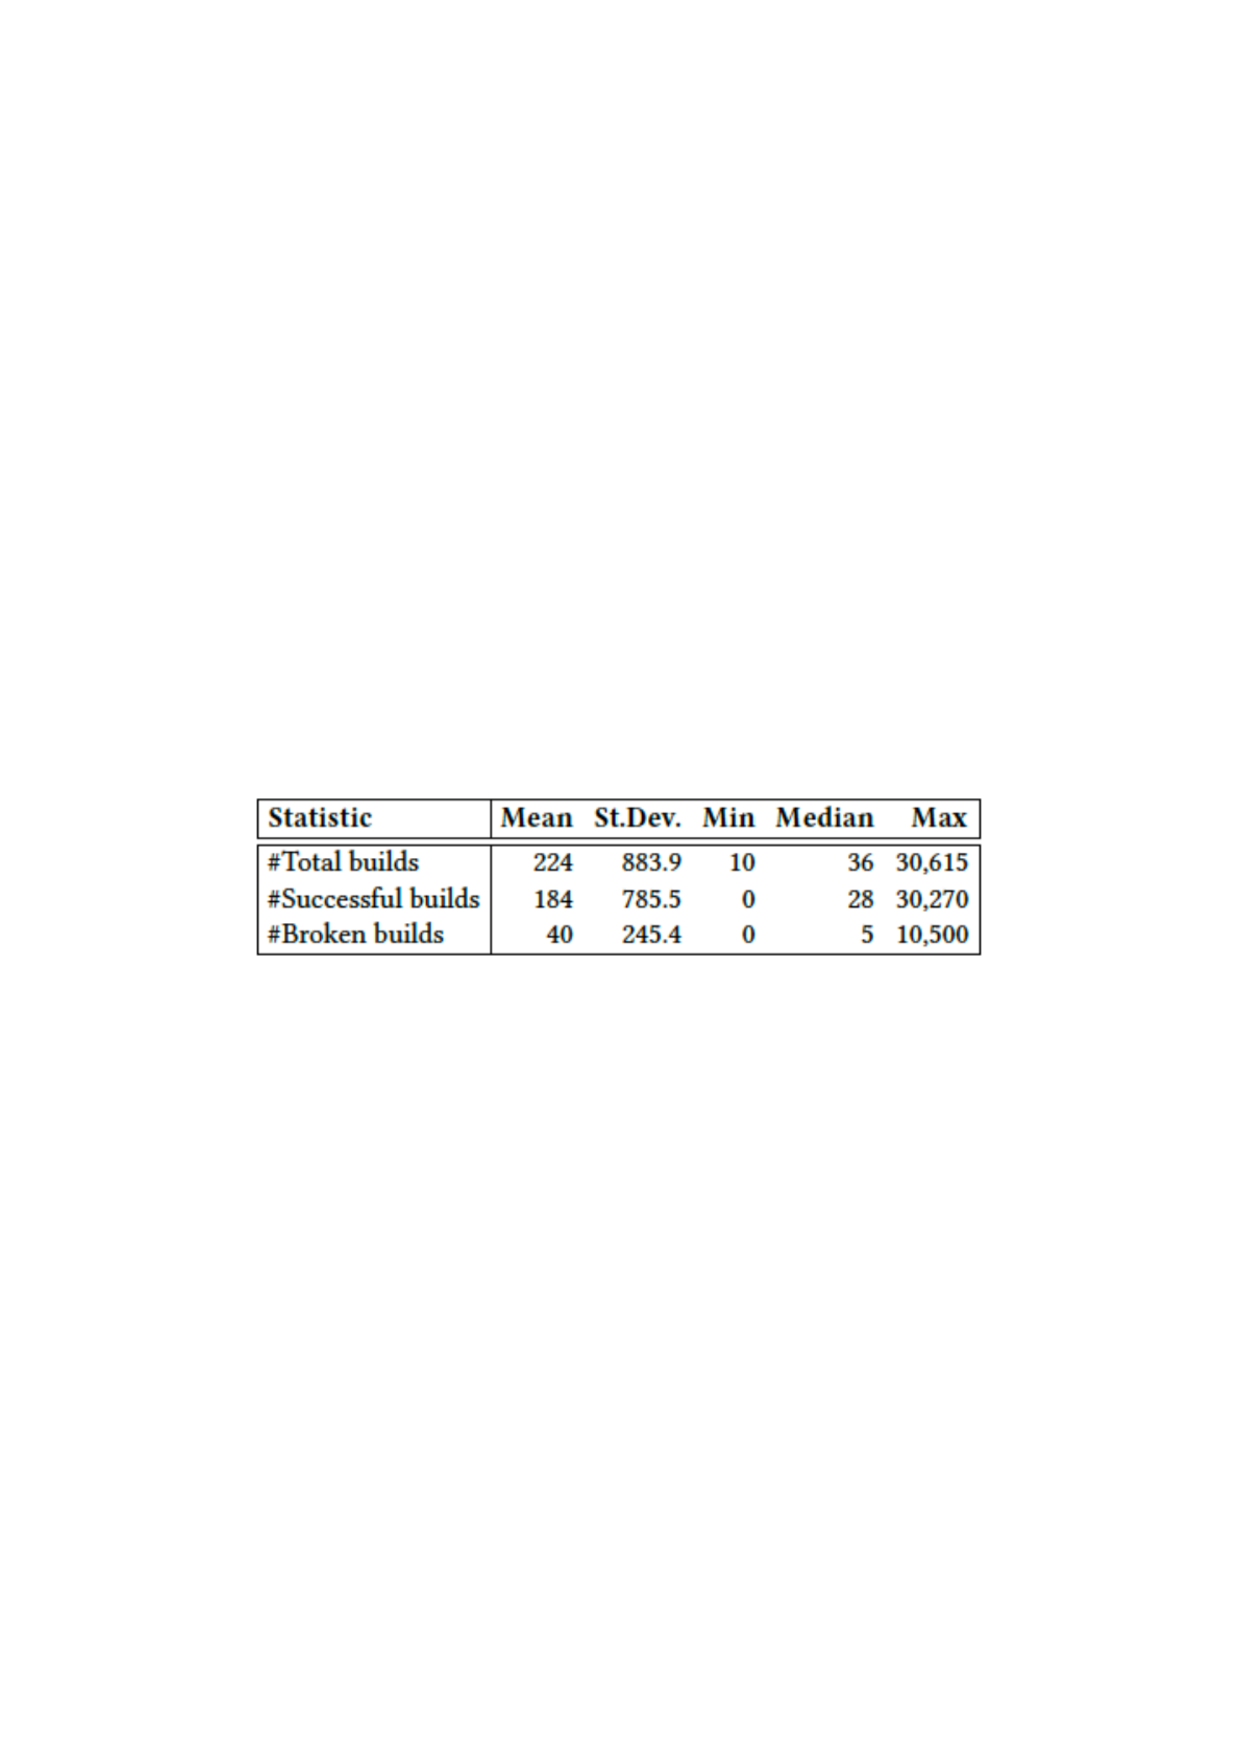
\includegraphics[width=0.9\linewidth, angle=0]{./thesis3/docker-build-data3.pdf}
    \label{fig:3_docker-build-data}
\end{table}

\subsection{データ処理}

\begin{figure}[t]
    \centering
    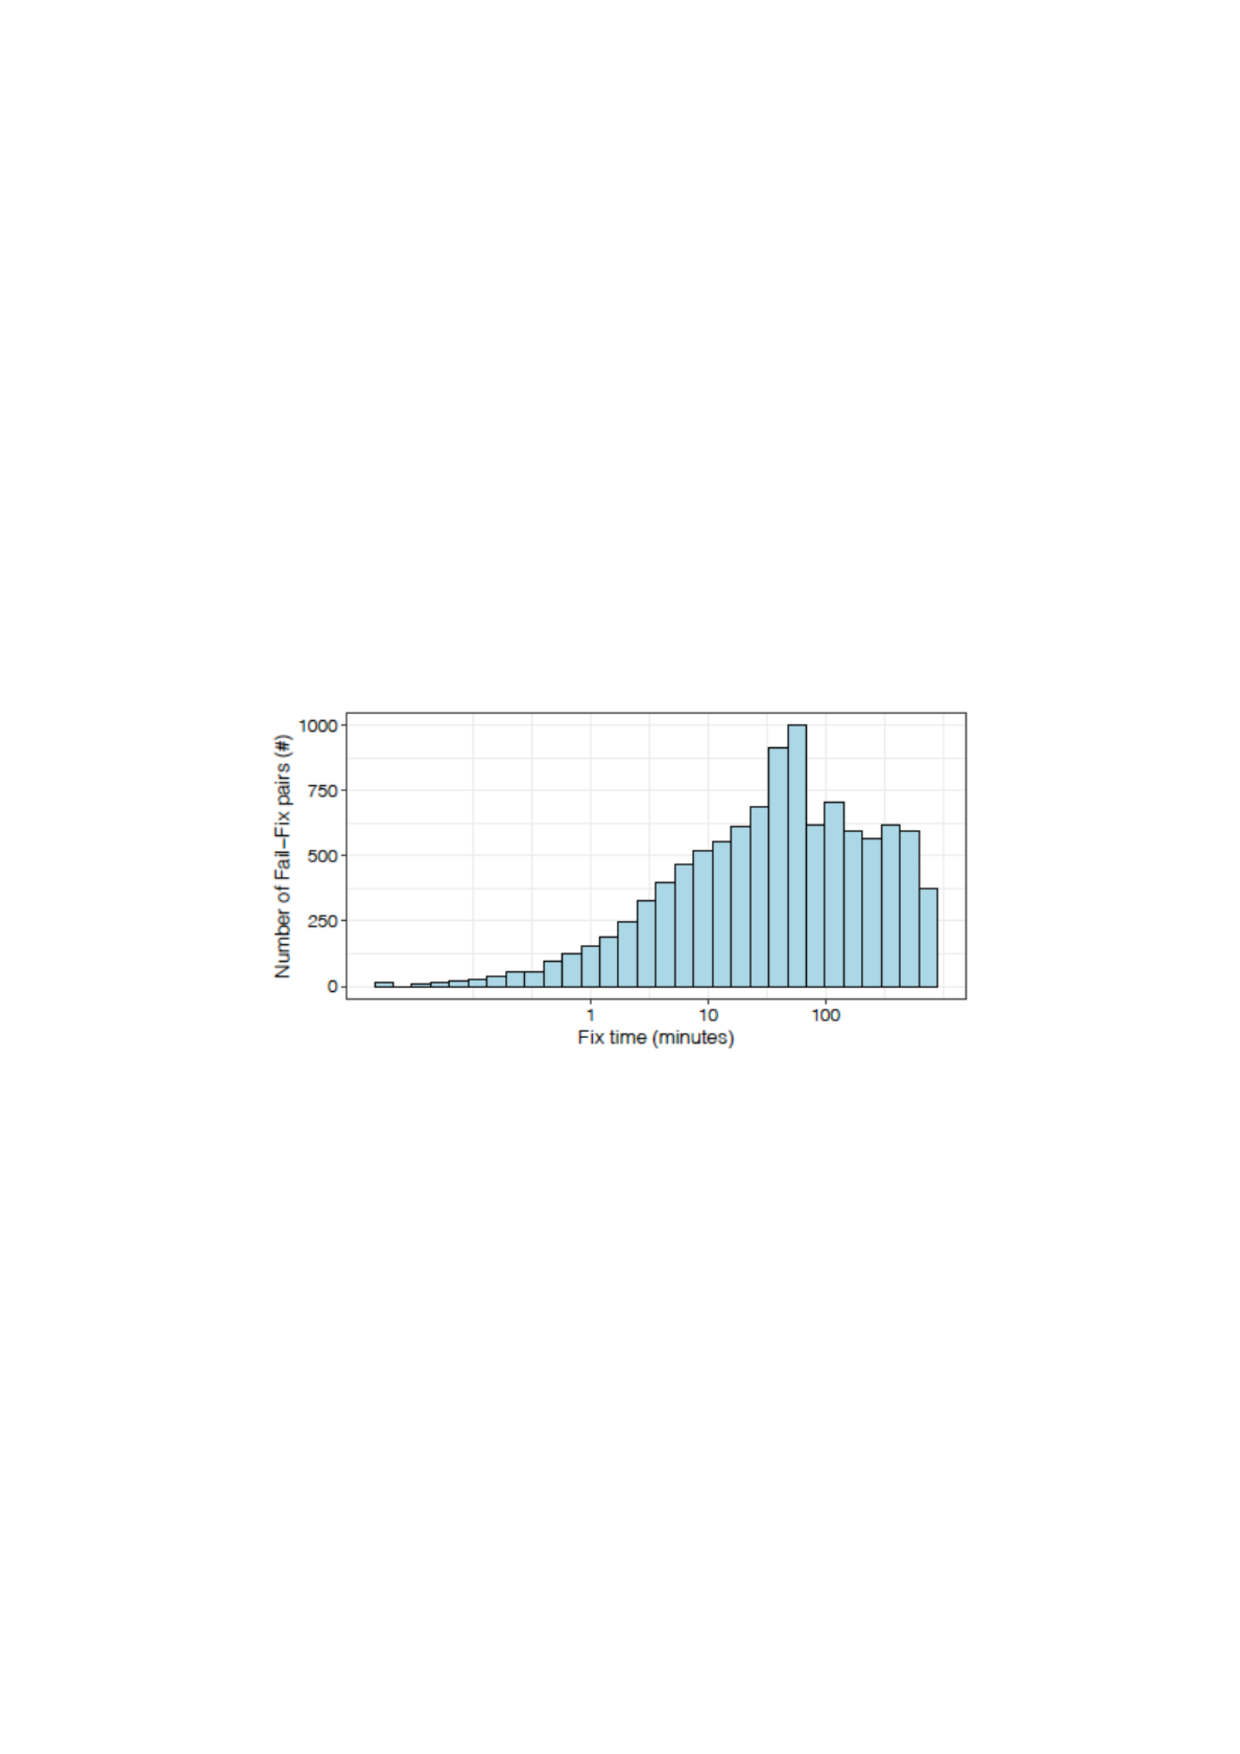
\includegraphics[width=0.9\linewidth, angle=0]{./thesis3/docker-build-failuer-number3.pdf}
    \caption{修正時間の分布}
    \label{fig:3_docker-build-failuer-number}
\end{figure}

\begin{figure}[t]
    \centering
    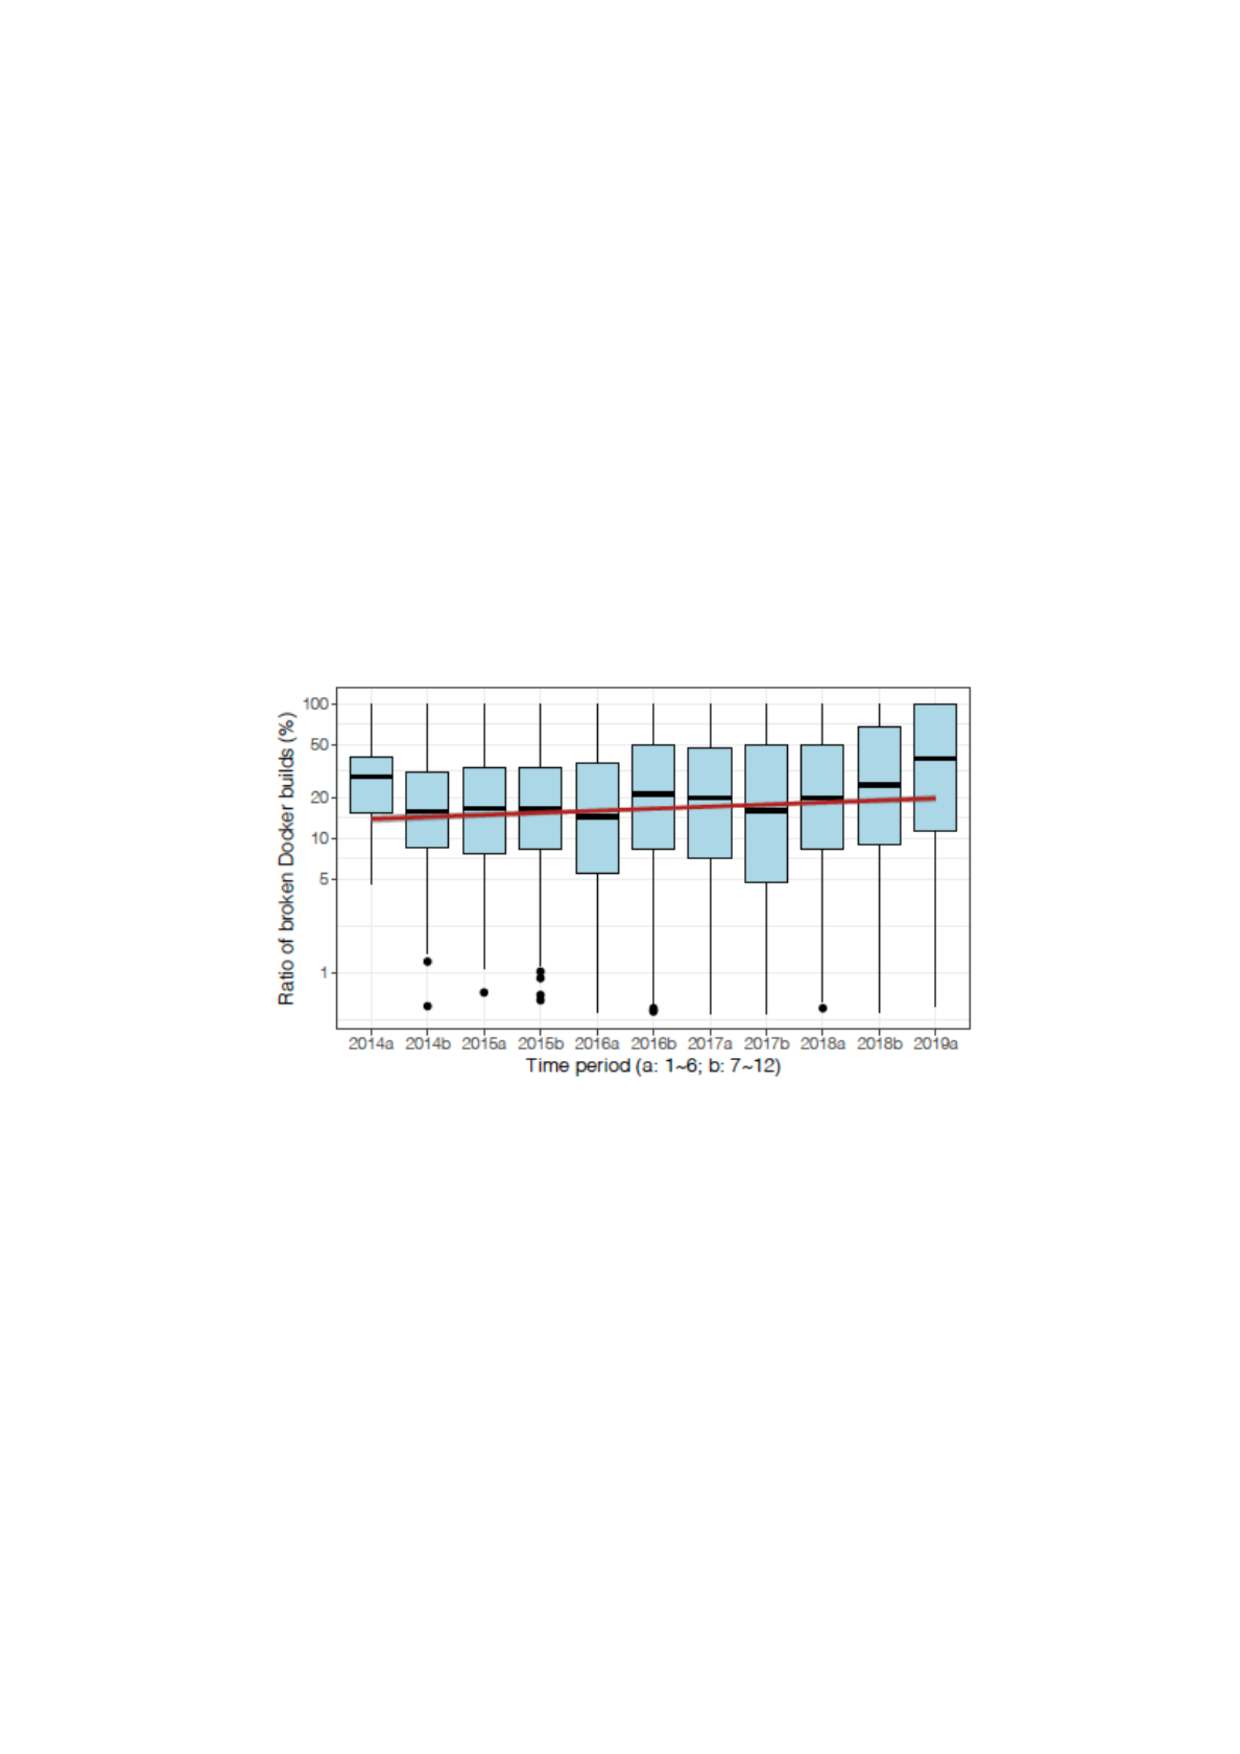
\includegraphics[width=0.9\linewidth, angle=0]{./thesis3/docker-build-failuer-ratio-period3.pdf}
    \caption{6ヶ月間のビルドの失敗率の分布}
    \label{fig:3_docker-build-failer-ratio-period}
\end{figure}

\begin{figure}[t]
    \centering
    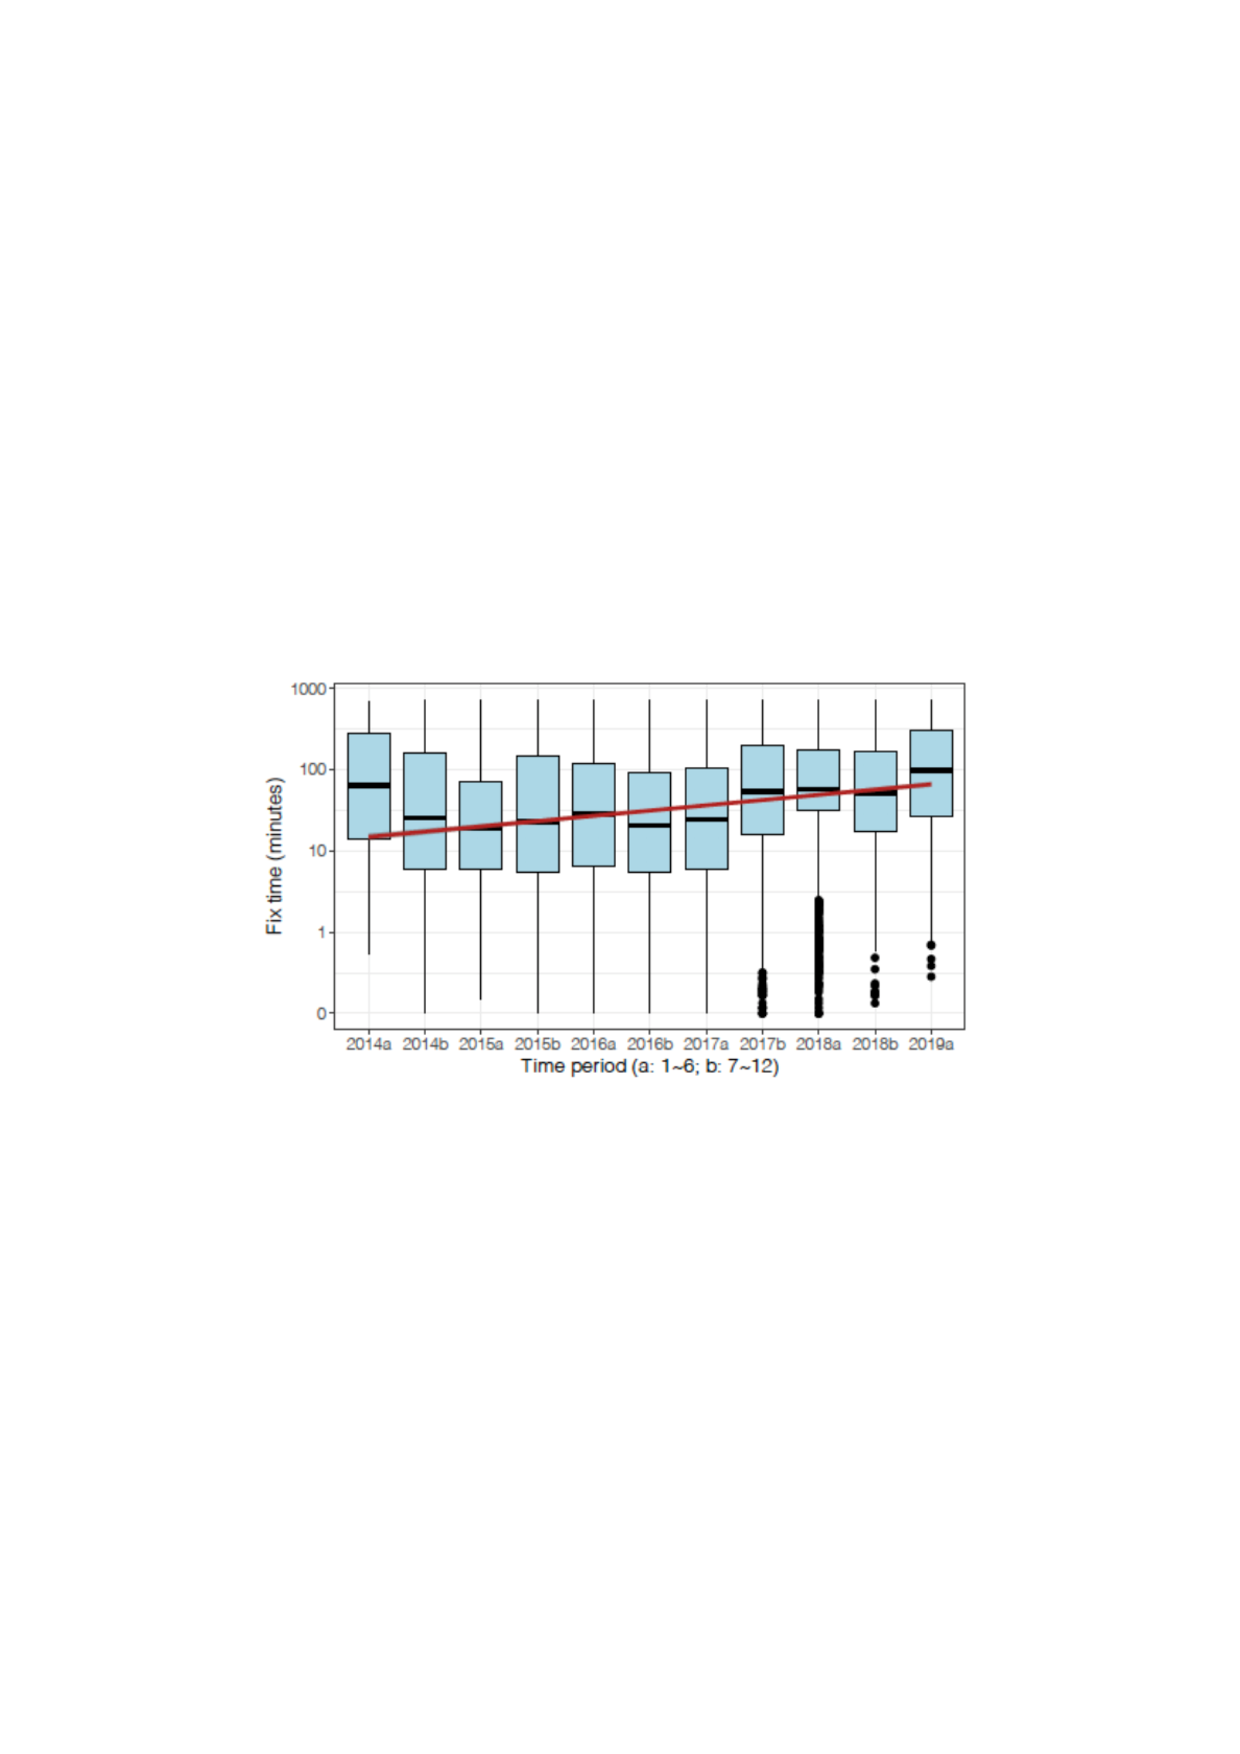
\includegraphics[width=0.9\linewidth, angle=0]{./thesis3/docker-build-fix-time-period3.pdf}
    \caption{6ヶ月間の修正時間の分布}
    \label{fig:3_docker-build-fix-time-period}
\end{figure}

RQ2についてビルドの修正時間にどれくらいの時間を要するかを分析するために,バグとその修正のペアの特定を行っている.

% 文献\cite{docker-failures}ではRabbaniら\cite{3-ref-5}が提案したバグとその修正のペアを特定する方法を用いている.

具体的には,ビルドが成功した直後に続く失敗したビルド(A)を発見し,次に発見する成功したビルド(B)のABのペアを,ビルドの失敗とその修正としている.ここで開発者のスケジュールが修正時間に影響しないように,修正時間が12時間を超えるものをフィルタリングしている.図\ref{fig:3_docker-build-failuer-number}にDockerビルドの修正時間の分布を示す.

% === RQ2の考察 =======
% 有効な10,566件のFail-Fixペアのうち、511件(4.8%)が1分未満、2,105件(19.9%)が1分から10分、4,511件(42.7%)が10分から100分、3,431件(32.5%)が100分以上の時間を要しています。
% 我々のデータセットでは、壊れたビルドの修正に平均124.5分(中央値:44.2分)かかり、これはGoogleの研究(12分未満)よりもはるかに長いです[7]。
% この差には、作業環境やツールなど多くの要因が関係していると考えられる。また、この差が大きいのは、Google が開発者の広範囲に影響を与えないように、開発者に障害発生時の迅速な対応を要求しているためと考えられる[11]。しかし、オープンソースプロジェクトの開発者がこのような規制を完全に遵守することは困難です。また、従来のビルドプロセスとは異なり、各Dockerビルドは、コードからパッケージング、テスト、クラウドレジストリへのプッシュまでのプロセスを完了させる必要があり、長い時間がかかる可能性があります。
% このため、開発者は最終的なビルド結果を見て不具合が修正されたかどうかを判断するために長い時間を待つことになり、Dockerビルドの不具合修正にマイナスの影響を与える可能性があります。そのため、開発者に潜在的なビルド結果(例えば、失敗か成功か、ビルドが失敗した場合の修正時間の予測など)を思い出させるためのビルド予測技術が必要とされています。
% % その結果、プロジェクトあたりの壊れたビルド数は、修正時間の中央値と正の相関があることがわかりました(スピアマンのrho=0.28、p<0.001)。このように、ビルド数が多いプロジェクトほど、修正時間が長くなることがわかりました。失敗が多すぎると、開発者の時間と集中力が散漫になり、その結果、困難な失敗や重要な失敗を時間内に修正することができないことがある。

また,RQ3についてDockerのビルドの失敗とその修正時間の,時間経過による関係性を調査するため,6ヶ月間の期間ごとにデータを集計する.その結果を図\ref{fig:3_docker-build-failer-ratio-period},図\ref{fig:3_docker-build-fix-time-period}に示す.



% \begin{figure}[t]
%     \centering
%     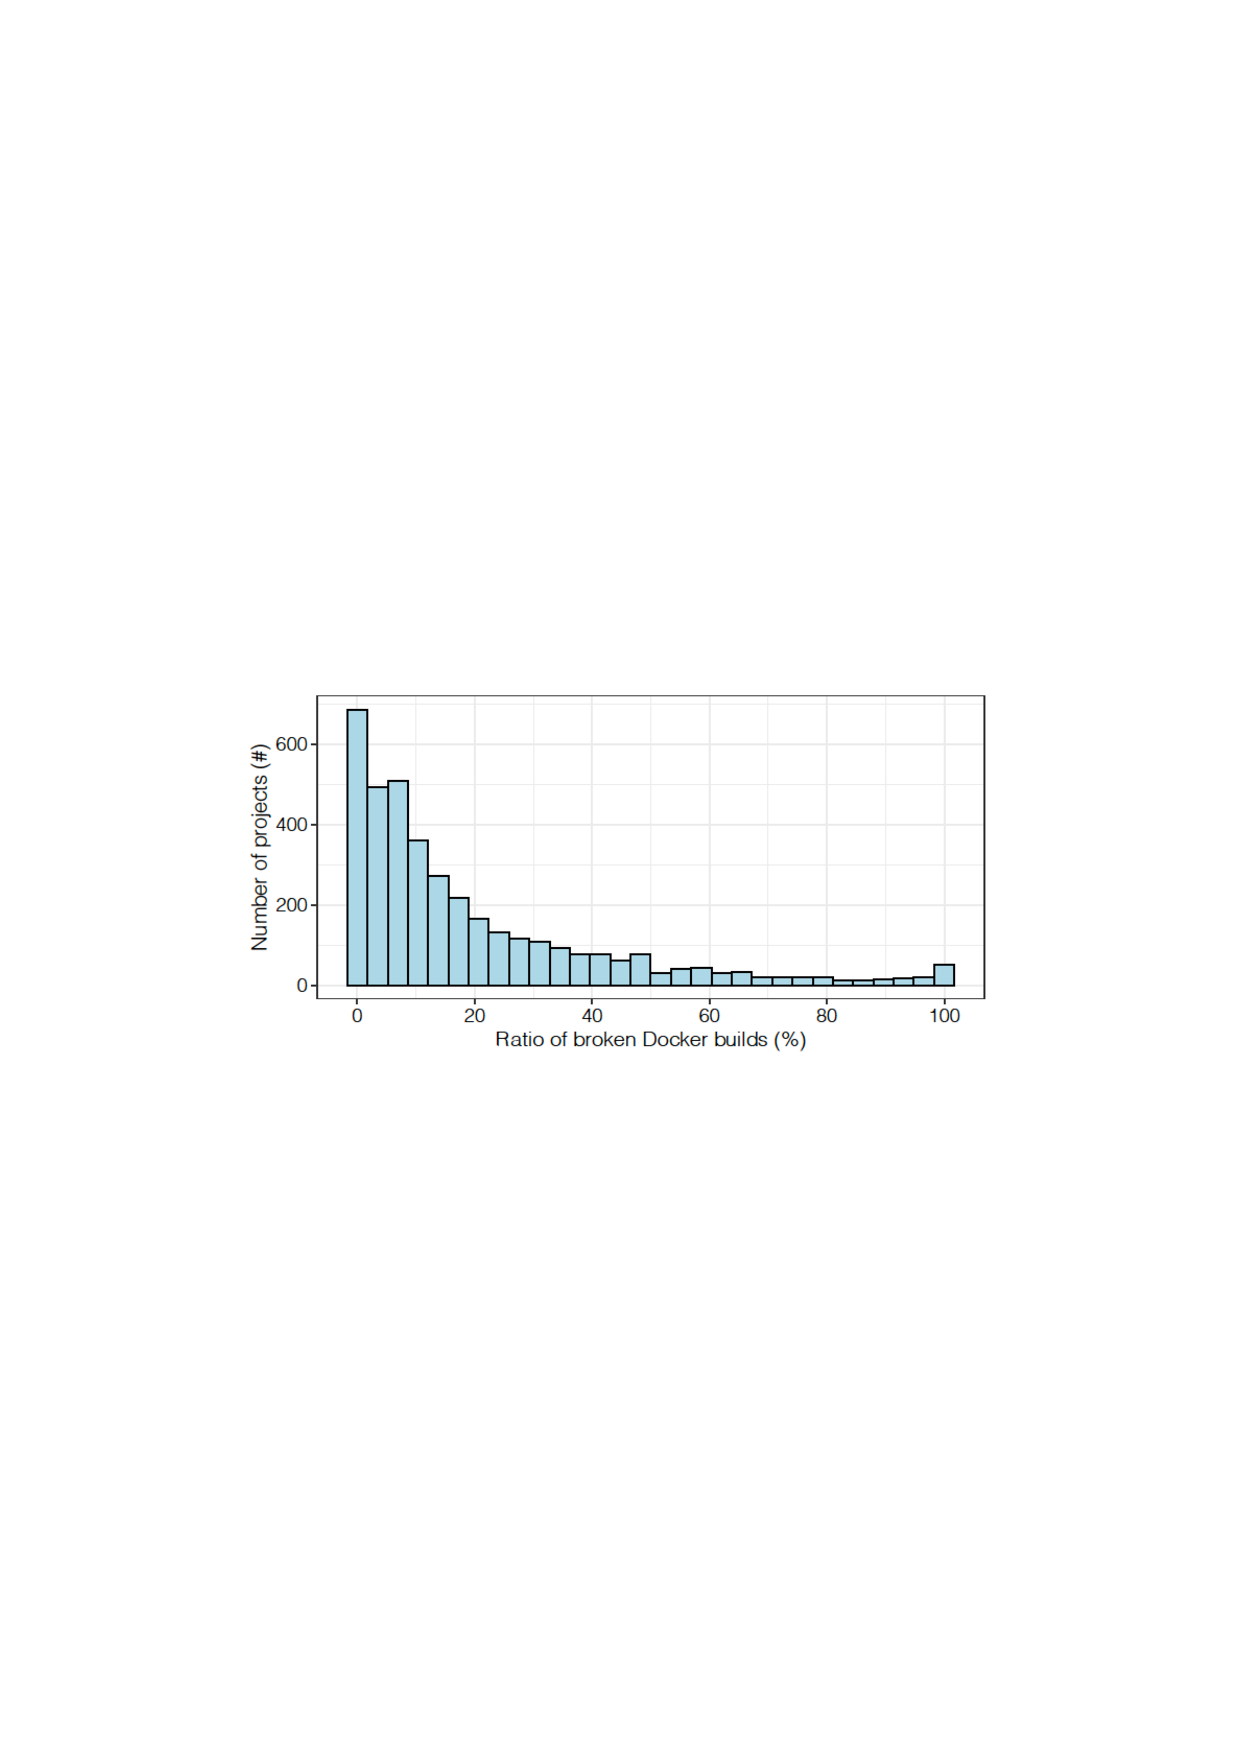
\includegraphics[width=0.9\linewidth, angle=0]{./thesis3/docker-build-number3.pdf}
%     \label{fig:3_docker-build-number}
%     \caption{ビルド失敗件数の分布}
% \end{figure}


\subsection{結果}
文献\cite{docker-failures}では,Docker環境におけるビルドの失敗事例について,大規模な実証実験を行っている.その結果,対象にした3,828件のプロジェクトにおいて,85.2\%のプロジェクトでビルドが発生しており,857,086件のビルドデータのうち17.8\%が失敗しているということが明らかになっている.また,31.5\%のプロジェクトにおいて,ビルドの20\%以上が失敗している.
% しかし,頻繁にビルドされているプロジェクトでは,ビルド失敗の割合は比較的低くなっている
失敗したビルドの修正時間については,平均124.5分,中央値が44.2分であり,ビルドの失敗が頻繁に発生するプロジェクトでは,その修正時間が長いという結果も示されている.この結果は従来のビルドプロセスよりも長い時間になっている.
文献\cite{docker-failures}では,Dockerのビルドは従来と異なりコードからパッケージング,テスト,クラウドへのデプロイまでのプロセスがあり,修正に長い時間がかかるために,ビルドの失敗が多いほど修正時間も長くなっていくと示唆している.
また,図\ref{fig:3_docker-build-failer-ratio-period},図\ref{fig:3_docker-build-fix-time-period}よりDockerのビルドが失敗する割合やその修正に要する時間は,時間の経過とともにどちらも増加する傾向があるということが示されている.

% 先行研究\cite{3-ref-12}では,Dockerのビルドにかかる遅延時間が時間の経過とともに増加する傾向があることが確認されている.時間,負荷のかかるビルドは,失敗率を高める可能性があり,さらにRQ2で示されたように,より多くのビルドの失敗数と修正時間には相関があることが示されている.文献\cite{docker-failures}ではこれらの要因により,ビルド失敗率と修正時間が時間の経過とともに増加する可能性があると示唆している.

文献\cite{docker-failures}より,Dockerにおいてビルドの失敗とその修正時間は時間の経過とともに長くなっていくことがわかり,その原因としてDockerにおける開発手法の知見が不足していることが考えられる.また同時に,Dockerfile内にビルドの失敗に関係するようなSATDコメントが含まれることが考えられ,SATDの返済について調査を行うことは,Dockerにおけるビルドの失敗や潜在するバグの問題を解決するのに有効であると考えられる.
\vspace{-1mm}
\section{まとめ}
第2章では5つの大規模なオープンソースプロジェクトにおけるSATDの解消期間や解消の割合についての調査結果,第3章ではSATD解消時のソースコードやコミットメッセージへの影響についての調査結果,第4章ではDockerにおけるビルドの失敗率とその修正期間についての調査結果を報告した.
Dcokerは比較的新しい技術であり,その開発手法が確立されていないことは,文献\cite{docker-failures}にて明確になっている.文献\cite{satd-real-removal},文献\cite{satd-real-removal}のようなSATDの削除に関する調査を行うことは,Dockerにおけるベストプラクティスな開発手法やSATD削除に関する知見の提供,開発支援を行うツールの作成につながると考えられる.
今後はこれらの調査手法や結果を参考に,DockerにおけるSATDの解消に関する調査を行っていく.


\vspace{-2mm}

\begin{thebibliography}{9}

\vspace{-3mm}

\bibitem{docker-satd}
東英明, まつ本真佑, \textit{et al.}, ``コンテナ仮想化技術におけるSelf-Admitted Technical Debtの調査" 電子情報通信学会技術研究報告, pp.25-30, 2020

\bibitem{satd-removal}
E.d.S.Maldonado, R.Abdalkareem, \textit{et al.}, ``An Empirical Study on the Removal of Self-Admitted Technical Debt." 2017 IEEE International Conference on Software Maintenance and Evolution (ICSME), pp.238-248, 2017

\bibitem{satd-real-removal}
F.Zampetti, A.Serebrenik, \textit{et al.}, ``Was Self-Admitted Technical Debt Removal a Real Removal? An In-Depth Perspective." 2018 IEEE/ACM 15th International Conference on Mining Software Repositories (MSR), pp.526-536, 2018

\bibitem{docker-failures}
Yiwen Wu, Yang Zhang, \textit{et al.}, ``An Empirical Study of Build Failures in the Docker Context." the 17th International Conference on Mining Software Repositories (MSR '20), pp.76–80, 2020

\bibitem{1-ref-25}
E.d.S.Maldonado, E.Shihab, \textit{et al.}, ``Using natural language processing to automatically detect self-admitted technical debt" IEEE Transactions on Software Engineering, pp.1044-1062, 2017

% ==== フォーマットが統一されていない ====
% \bibitem{docker-satd}
% 東英明,まつ本真佑, 亀井靖高 and 楠本真二, "コンテナ仮想化技術におけるSelf-Admitted Technical Debtの調査" 電子情報通信学会技術研究報告, 2020, pp. 25-30.

% \bibitem{satd-removal}
% E.D.S.Maldonado, R.Abdalkareem, E.Shihab and A.Serebrenik, "An Empirical Study on the Removal of Self-Admitted Technical Debt," 2017 IEEE International Conference on Software Maintenance and Evolution (ICSME), Shanghai, 2017, pp. 238-248, doi: 10.1109/ICSME.2017.8.

% \bibitem{satd-real-removal}
% F. Zampetti, A. Serebrenik and M. Di Penta, "Was Self-Admitted Technical Debt Removal a Real Removal? An In-Depth Perspective," 2018 IEEE/ACM 15th International Conference on Mining Software Repositories (MSR), Gothenburg, 2018, pp. 526-536.

% \bibitem{docker-failures}
% Yiwen Wu, Yang Zhang, Tao Wang, and Huaimin Wang. 2020. An Empirical Study of Build Failures in the Docker Context. In Proceedings of the 17th International Conference on Mining Software Repositories (MSR '20). Association for Computing Machinery, New York, NY, USA, 76–80. DOI:https://doi.org/10.1145/3379597.3387483

% \bibitem{1-ref-25}
% E.Maldonado, E.Shihab, and N.Tsantalis. Using natural language processing to automatically detect self-admitted technical debt. IEEE Transactions on Software Engineering, page to appear, 2017.

% =================================== 

% \bibitem{1-ref-29}
% A.Potdar and E.Shihab. An exploratory study on self-admitted technical debt. In International Conference on Software Maintenance and Evolution, pages 91–100. IEEE Computer Society, 2014.

% \bibitem{1-ref-37}
% T.Punter, M.Ciolkowski, B.Freimut, and I.John. Conducting online surveys in software engineering. In International Symposium on Empirical Software Engineering., pages 80–88. IEEE, 2003.

% \bibitem{3-ref-5}
% Noam Rabbani, Michael S Harvey, Sadnan Saquif, Keheliya Gallaba, and Shane McIntosh. 2018. Revisiting" Programmers’ Build Errors" in the Visual Studio Context. In 2018 IEEE/ACM 15th International Conference on Mining Software Repositories (MSR). IEEE, 98–101

% \bibitem{3-ref-12}
% Yang Zhang, Bogdan Vasilescu, Huaimin Wang, and Vladimir Filkov. 2018. One size does not fit all: an empirical study of containerized continuous deployment workflows. In Proceedings of the 2018 26th ACMJoint Meeting on European Software Engineering Conference and Symposium on the Foundations of Software Engineering (ESEC/FSE). ACM, 295–306.

% =============================================


\end{thebibliography}
\vspace{-5mm}

\begin{list}{}{\labelwidth=18mm \itemindent=8mm}
	\renewcommand{\makelabel}{\normalsize}
	\item[\quad 講演者\hfill]: 新堂 風 
	\item[\quad 指導教員\hfill]: 亀井 靖高 准教授
	\item[\quad 講演日時\hfill]: 2020年12月14日(月)16:40~17:25
	\item[\quad 講演場所\hfill]: Teams
\end{list}

\end{document}
